\section{Resultados}\label{sec:resultados}
A continuación, se presentan los casos de estudio que se han realizado para diferentes simulaciones del juego
de la vida en dos y tres dimensiones, y sus respectivos resultados.
Para cada caso, se detallan los parámetros de entrada fijos utilizados, seguido de una o más figuras en el que
se muestra la evolución del sistema en cada paso temporal en valores extremos, y finalmente, un análisis del
observable en función de la densidad de celdas vivas en el dominio inicial.

\subsection{Conway en 2D}\label{subsec:conway-en-2d}

Como primer modelo, se ha estudiado el reconocido juego de la vida de Conway en dos dimensiones.
Para ello, se fija los siguientes parámetros de entrada:

\begin{itemize}
    \item $border = (0, 0) \times (100, 100)$
    \item $condition = MOORE$
    \item $r = 1$
    \item $shouldKeepAlive = [2, 3]$
    \item $shouldRevive = [3]$
    \item $initialDomainProportion = 0.16$
\end{itemize}
Variando el parámetro $initialLiveCellsProportion$ entre 0.1 y 0.9, se ha analizado la cantidad de celdas vivas
a lo largo de los pasos temporales.
\begin{figure}[H]
    \centering
    \includegraphics[width=0.6\linewidth]{conway2d/size_i10}
    \caption{Cantidad de celdas vivas en el tiempo del sistema de Conway con $initialLiveCellsProportion = 0.1$}
    \label{fig:conway2d_i10}
\end{figure}
\begin{figure}[H]
    \centering
    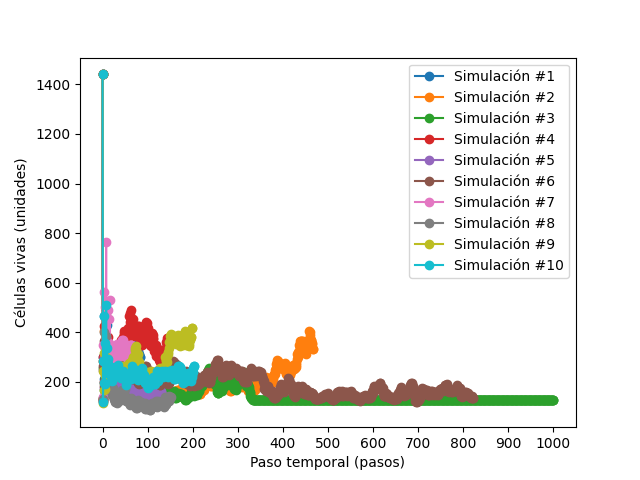
\includegraphics[width=0.6\linewidth]{conway2d/size_i90}
    \caption{Cantidad de celdas vivas en el tiempo del sistema de Conway con $initialLiveCellsProportion = 0.9$}
    \label{fig:conway2d_i90}
\end{figure}

De igual forma, se ha analizado la distancia de la celda viva más lejana al centro de la matriz en función del
paso temporal.

\begin{figure}[H]
    \centering
    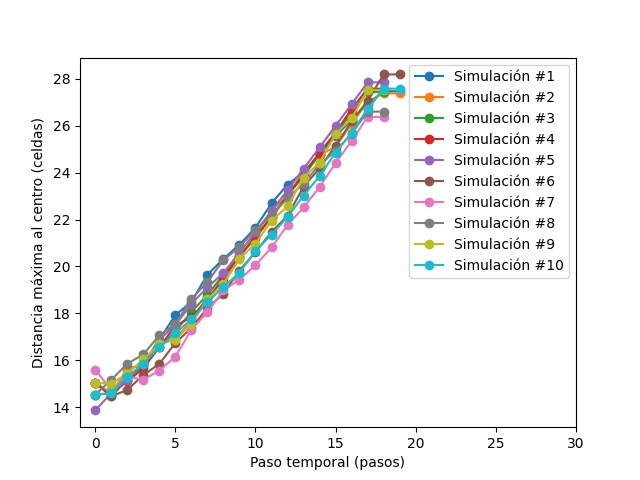
\includegraphics[width=0.6\linewidth]{conway2d/distance_i10}
    \caption{Distancia de la celda viva más lejana al centro en función del tiempo con $initialLiveCellsProportion = 0.1$}
    \label{fig:conway2d_d10}
\end{figure}
\begin{figure}[H]
    \centering
    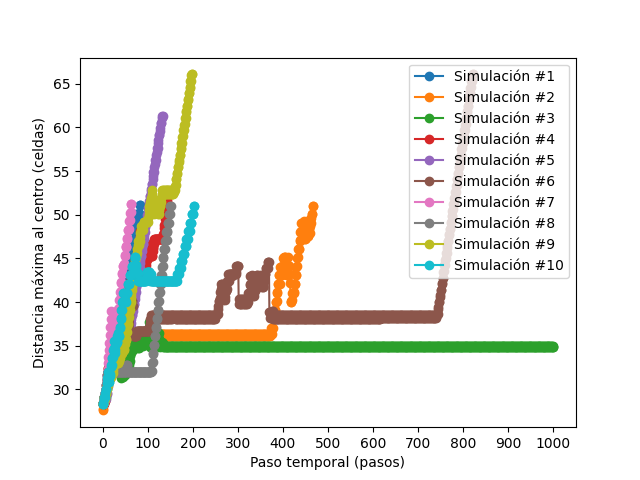
\includegraphics[width=0.6\linewidth]{conway2d/distance_i90}
    \caption{Distancia de la celda viva más lejana al centro en función del tiempo con $initialLiveCellsProportion = 0.9$}
    \label{fig:conway2d_d90}
\end{figure}

Como se puede apreciar, el sistema alcanza el equilibrio antes del paso temporal 900, por lo que se hace el análisis
del observable en el paso temporal mencionado.
Para este modelo, en función de la densidad de celdas vivas en el dominio inicial, se ha observado la cantidad de celdas vivas,
la pendiente de crecimiento de la cantidad de celdas vivas







\subsection{Cuarentena en 2D}\label{subsec:cuarentena-2D}

El objetivo de este sistema es limitar el crecimiento en cantidad de celdas vivas a únicamente la sección inicial o una subparte de esta. Para ello
se utilizaron los siguientes parámetros:

\begin{itemize}
    \item $border = (0, 0) \times (100, 100)$
    \item $condition = MOORE$
    \item $r = 1$
    \item $shouldKeepAlive = [1, 2, 3, 4, 5, 6, 7, 8]$
    \item $shouldRevive = [4, 5, 6, 7, 8]$
    \item $initialDomainProportion = 0.16$
\end{itemize}

2.4.1 Para cada input o parámetro a estudiar, primero mostrar una animación característica del 
sistema (pueden ser dos, con dos valores extremos del input para ver ejemplos de distintos 
comportamientos). La idea de esto es ilustrar la dinámica del sistema para situar el contexto de los 
resultados a mostrar. Acuerdense de poner un fotograma representativo y después el link a youtube 

A continuación se puede observar una animación característica del sistema con un input de 0.5:

\begin{figure}[H]
    \centering
    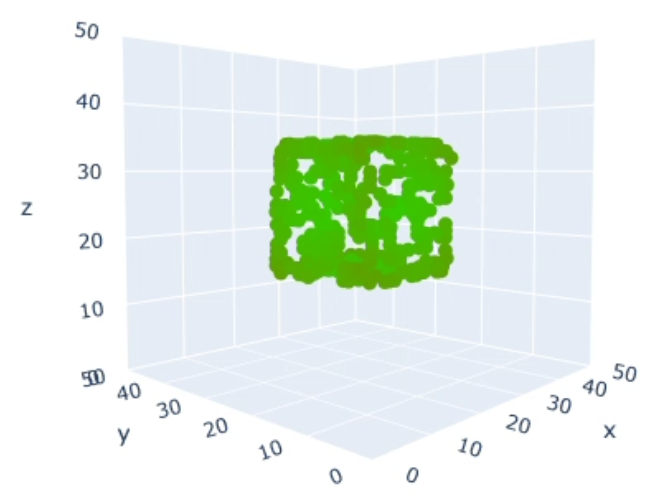
\includegraphics[width=0.6\linewidth]{cuarentena2d/thumbnail_i50}
    \caption{Fotograma de la animación de Cuarentena con $initialLiveCellsProportion = 0.5$}
    \label{fig:thumbnailcuarentena2d_i50}
\end{figure}

Enlace a la animación completa: https://youtu.be/hAECaws6P90

2.4.2 Luego mostrar una figura del observable o métrica (que se calcula a partir de los outputs 
directos de la simulación) en función del tiempo. Explicar entonces cual será el escalar que 
caracteriza ese proceso (por ejemplo el promedio de la evolución temporal en el estado 
estacionario, la tasa de crecimiento, etc.). Solo mostrar evoluciones típicas, de valores extremos 
del rango de parámetros, para validar las definiciones de los observables. Las evoluciones en sí 
no son los resultados definitivos, por lo tanto no deben ser extenso lo que se muestre de las 
mismas solo para justificar el observable (escalar) que se calculará a partir de estas.

A diferencia de los otros sistemas, en este no solo se varió el parámetro $initialLiveCellsProportion$ entre 0.1 y 0.9 con un paso de 0.1, 
sino que además se agregaron corridas con el parámetro valiendo 0.05 y 0.15.

A continuación podemos observar cómo evoluciona la cantidad de celdas vidas en función del tiempo para disitntos valores del parámetro $initialLiveCellsProportion$

\begin{figure}[H]
    \centering
    \includegraphics[width=0.6\linewidth]{cuarentena2d/size_i10}
    \caption{Cantidad de celdas vivas en el tiempo del sistema de Cuarentena con $initialLiveCellsProportion = 0.1$}
    \label{fig:cuarentena2d_i10}
\end{figure}
\begin{figure}[H]
    \centering
    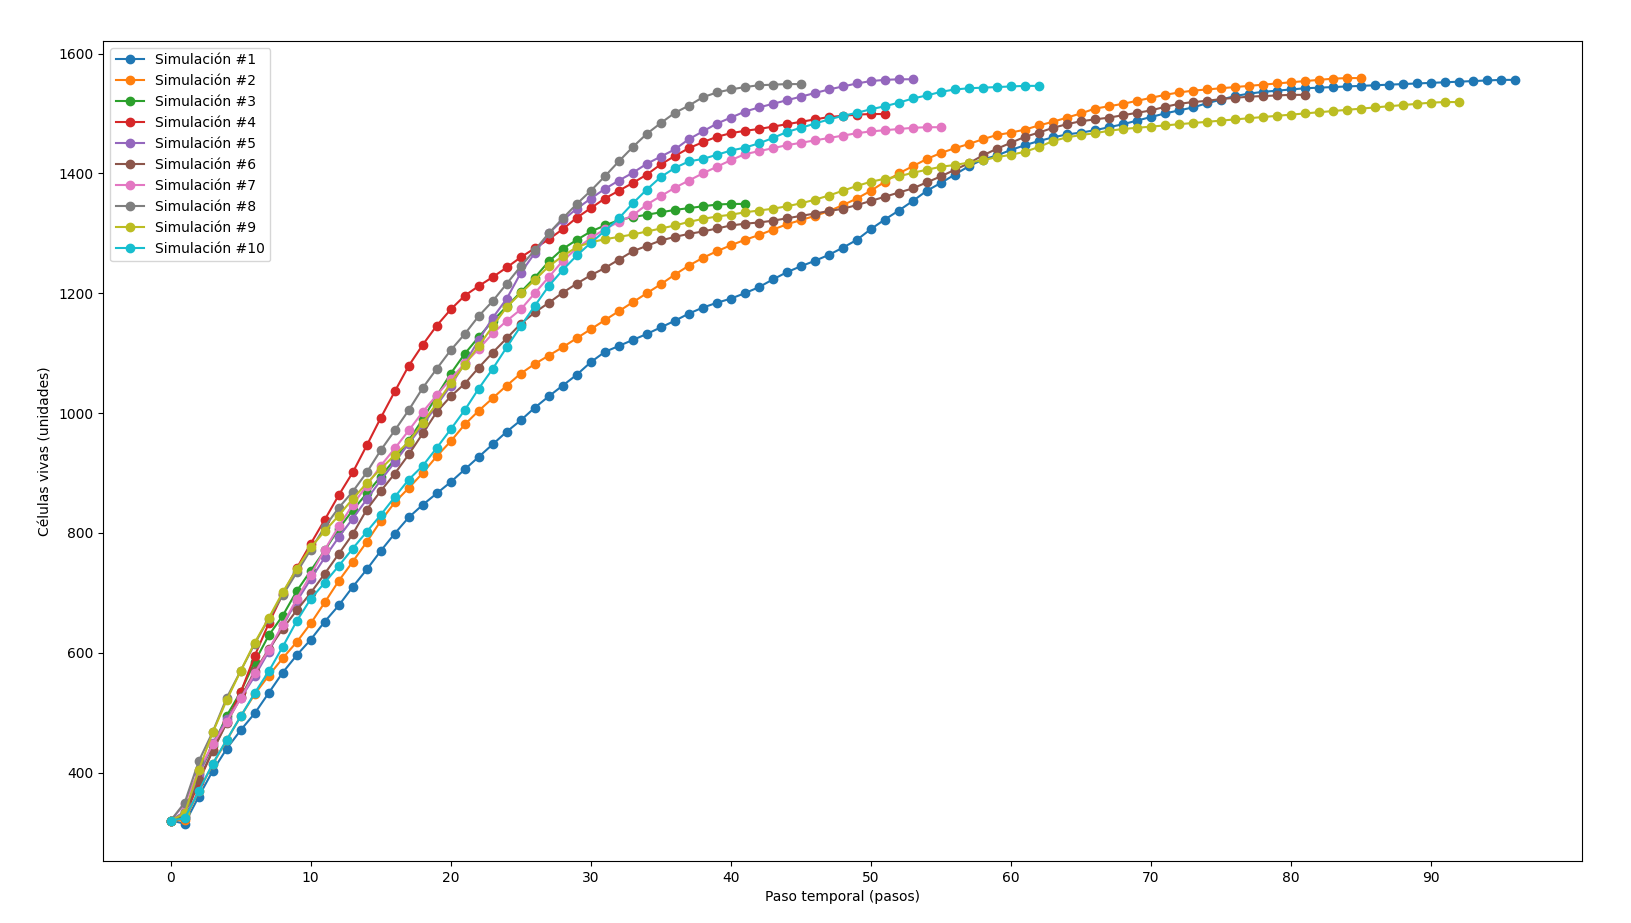
\includegraphics[width=0.6\linewidth]{cuarentena2d/size_i20}
    \caption{Cantidad de celdas vivas en el tiempo del sistema de Cuarentena con $initialLiveCellsProportion = 0.2$}
    \label{fig:cuarentena2d_i20}
\end{figure}
\begin{figure}[H]
    \centering
    \includegraphics[width=0.6\linewidth]{cuarentena2d/size_i80}
    \caption{Cantidad de celdas vivas en el tiempo del sistema de Cuarentena con $initialLiveCellsProportion = 0.8$}
    \label{fig:cuarentena2d_i80}
\end{figure}

La distancia de la celda viva más lejana al centro en función del tiempo es prácticamente idéntica para todos los inputs utilizados.

Lo interesante de este sistema no es la cantidad de celdas vivas en el momento de equilibrio debido a que si utilizamos $initialLiveCellsProportion$
por lo que hacemos hincapie en el crecimiento de cantidad de células vivas.

SUPONGO QUE HAY QUE HABLAR ACERCA DE CÓMO SE HIZO EL CÁLCULO DE CRECIMIENTO 


2.4.3 Después presentar la figura del input vs. observable, con promedio y barras de error o tablas 
con promedio y error. 

A continuación observamos el análisis del observable

\begin{figure}[H]
    \centering
    \includegraphics[width=0.6\linewidth]{cuarentena2d/observable}
    \caption{Pendiente de crecimiento de cantidad de celdas vivas en función del input para el sistema Cuarentena 2D}
    \label{fig:cuarentena2d_observable}
\end{figure}







\subsection{Expansión Circular en 2D}\label{subsec:expansion-circular-2D}

El objetivo de este sistema es obtener un crecimiento similar en todas las direcciones. Para ello se utilizaron los siguientes parámetros:

\begin{itemize}
    \item $border = (0, 0) \times (100, 100)$
    \item $condition = MOORE$
    \item $r = 1$
    \item $shouldKeepAlive = [0, 1, 4, 5, 6, 7, 8]$
    \item $shouldRevive = [2, 3]$
    \item $initialDomainProportion = 0.16$
\end{itemize}

2.4.1 Para cada input o parámetro a estudiar, primero mostrar una animación característica del 
sistema (pueden ser dos, con dos valores extremos del input para ver ejemplos de distintos 
comportamientos). La idea de esto es ilustrar la dinámica del sistema para situar el contexto de los 
resultados a mostrar. Acuerdense de poner un fotograma representativo y después el link a youtube 

A continuación se puede observar una animación característica del sistema con un input de 0.6:

\begin{figure}[H]
    \centering
    \includegraphics[width=0.6\linewidth]{circular2d/thumbnail}
    \caption{Fotograma de la animación de Expansión Circular con $initialLiveCellsProportion = 0.6$}
    \label{fig:thumbnailcircular2d_i60}
\end{figure}

Enlace a la animación completa: https://youtu.be/AIikxHN6VO4

2.4.2 Luego mostrar una figura del observable o métrica (que se calcula a partir de los outputs 
directos de la simulación) en función del tiempo. Explicar entonces cual será el escalar que 
caracteriza ese proceso (por ejemplo el promedio de la evolución temporal en el estado 
estacionario, la tasa de crecimiento, etc.). Solo mostrar evoluciones típicas, de valores extremos 
del rango de parámetros, para validar las definiciones de los observables. Las evoluciones en sí 
no son los resultados definitivos, por lo tanto no deben ser extenso lo que se muestre de las 
mismas solo para justificar el observable (escalar) que se calculará a partir de estas.


Variando el parámetro $initialLiveCellsProportion$ entre 0.1 y 0.9 con un step de 0.1, se ha analizado la cantidad de celdas vivas en función
del tiempo.

\begin{figure}[H]
    \centering
    \includegraphics[width=0.6\linewidth]{circular2d/size_i10}
    \caption{Cantidad de celdas vivas en el tiempo del sistema de Expansión Circular con $initialLiveCellsProportion = 0.1$}
    \label{fig:circular2d_i10}
\end{figure}
\begin{figure}[H]
    \centering
    \includegraphics[width=0.6\linewidth]{circular2d/size_i80}
    \caption{Cantidad de celdas vivas en el tiempo del sistema de Expansión Circular con $initialLiveCellsProportion = 0.8$}
    \label{fig:circular2d_i80}
\end{figure}


Es posible visualizar que con ambos parámetros la simulación termina después de 33 pasos, esto se debe a que con este sistema, la simulación
siempre termina por haber llegado al borde. Por lo cual no es de interés analizar la distancia al centro de la celda viva más lejana, ya que
crece de manera lineal sin importar el valor de $initialLiveCellsProportion$.

Por otro lado, sí es interesante utilizar como observable la cantidad de celdas vivas en el instante final de la simulación, a continuación se
grafica este mismo en función del valor de $initialLiveCellsProportion$

2.4.3 Después presentar la figura del input vs. observable, con promedio y barras de error o tablas 
con promedio y error. 


\begin{figure}[H]
    \centering
    \includegraphics[width=0.6\linewidth]{circular2d/observable}
    \caption{Cantidad de celdas vivas en función del input para el sistema Expansión Circular}
    \label{fig:circular2d_observable}
\end{figure}






\subsection{Expansión Cúbica}\label{subsec:cubito-3D}

El objetivo de este sistema es crecer en cada paso 1 posición más alejada del centro, pero sin que la cantidad de celdas vivas crezca en todos los pasos.

\begin{itemize}
    \item $border = (0, 0) \times (100, 100)$
    \item $condition = MOORE$
    \item $r = 1$
    \item $shouldKeepAlive = [1, 2, 3, 4, 5, 6, 7, 8]$
    \item $shouldRevive = [4, 5, 6, 7, 8]$
    \item $initialDomainProportion = 0.16$
\end{itemize}


A continuación se puede observar una animación característica del sistema con un input de 0.9:

\begin{figure}[H]
    \centering
    \includegraphics[width=0.6\linewidth]{cubo3d/thumbnail}
    \caption{Fotograma de la animación de Expansión Cúbica con $initialLiveCellsProportion = 0.9$}
    \label{fig:thumbnailcubo3d_i90}
\end{figure}

Enlace a la animación completa: https://youtu.be/Zu9bqnto0ak


2.4.2 Luego mostrar una figura del observable o métrica (que se calcula a partir de los outputs 
directos de la simulación) en función del tiempo. Explicar entonces cual será el escalar que 
caracteriza ese proceso (por ejemplo el promedio de la evolución temporal en el estado 
estacionario, la tasa de crecimiento, etc.). Solo mostrar evoluciones típicas, de valores extremos 
del rango de parámetros, para validar las definiciones de los observables. Las evoluciones en sí 
no son los resultados definitivos, por lo tanto no deben ser extenso lo que se muestre de las 
mismas solo para justificar el observable (escalar) que se calculará a partir de estas.


Variando el parámetro $initialLiveCellsProportion$ entre 0.1 y 0.9 con un step de 0.1, se ha analizado la cantidad de celdas vivas en función
del tiempo.

\begin{figure}[H]
    \centering
    \includegraphics[width=0.6\linewidth]{cubo3d/size_i10}
    \caption{Cantidad de celdas vivas en el tiempo del sistema de Expansión Cúbica con $initialLiveCellsProportion = 0.1$}
    \label{fig:cubo3d_i10}
\end{figure}
\begin{figure}[H]
    \centering
    \includegraphics[width=0.6\linewidth]{cubo3d/size_i80}
    \caption{Cantidad de celdas vivas en el tiempo del sistema de Expansión Cúbica con $initialLiveCellsProportion = 0.8$}
    \label{fig:cubo3d_i80}
\end{figure}


Es posible visualizar que con ambos parámetros la simulación termina después de 19 pasos, esto se debe a que con este sistema, la simulación
siempre termina por haber llegado al borde. Por lo cual no es de interés analizar la distancia al centro de la celda viva más lejana, ya que
crece de manera lineal sin importar el valor de $initialLiveCellsProportion$.

Debido a la naturaleza del crecimiento resulta interesante analizar la pendiente de crecimiento en función del input.

2.4.3 Después presentar la figura del input vs. observable, con promedio y barras de error o tablas 
con promedio y error. 


\begin{figure}[H]
    \centering
    \includegraphics[width=0.6\linewidth]{cubo3d/observable}
    \caption{Pendiente de crecimiento de cantidad de celdas vivas en función del input para el sistema Expansión Circular}
    \label{fig:cubo3d_observable}
\end{figure}

